\documentclass[10pt,letterpaper]{article}
\usepackage[margin=0.75in]{geometry}
\usepackage[T1]{fontenc}
\usepackage[utf8]{inputenc}
\usepackage{lmodern}
\usepackage{amsmath,amssymb}
\usepackage{booktabs}
\usepackage{tabularx}
\usepackage{array}
\usepackage{graphicx}
\usepackage[font=small,labelfont=bf,skip=3pt]{caption}
\usepackage{enumitem}
\usepackage{microtype}
\usepackage[hidelinks]{hyperref}
\usepackage{xcolor}
\usepackage{parskip}
\usepackage{float}
\setlength{\parskip}{4pt}
\setlist{nosep,leftmargin=*}
\graphicspath{{../figures/}}
\newcommand{\lmax}{\lambda_{\max}}
\newcommand{\lmin}{\lambda_{\min}}
\newcommand{\M}{\,\mathrm{M}}
\newcolumntype{L}{>{\raggedright\arraybackslash}X}
\renewcommand{\arraystretch}{1.08}
\captionsetup[table]{skip=2pt}

\title{\vspace{-1.6em}CS 312 --- Assignment 3: Optimization 2\vspace{-0.4em}}
\author{Sandra Yang (\texttt{aleyang})}
\date{\vspace{-0.6em}}

\begin{document}
\maketitle
\vspace{-2em}

\paragraph{Setup.} Code: \texttt{experiments/a3\_optimization/} on branch \texttt{a3-experiments} of the fork \texttt{birdhumming/assignments}. Runs: W\&B project \texttt{assignments}, entity \texttt{aleyang-stanford-university}, tags \texttt{a3-*}. All training ran on Modal H100s, at most two at a time. The Problem~4 checkpoints are the course-supplied AdamW and SGD runs; we measured them and never retrained them. %GPUHOURS%

\paragraph{How to read the numbers.} ``Loss'' is validation loss in nats of the course d8 model (8 layers, width 512, batch 64, AdamW with $\beta=(0.9,0.95)$, weight decay 0.1) unless a problem says otherwise. From Assignment~1, the seed to seed standard deviation of this model's final loss is about 0.002. A gap below 0.005 is noise. A gap of 0.01 is small but real. A gap of 0.1 separates two regimes.

%=====================================================================
\section{Mode connectivity}
%P1%

%=====================================================================
\section{River valley dynamics}

\subsection*{(a) Schedules at equal tokens}

Every run trains the d8 model on 614M tokens with 3\% warmup. The schedules differ only in what happens after warmup. Linear decay, cosine decay and warmup-stable-decay with a 20\% decay tail (wsd0.2) all go to zero at the end. The constant schedule stays at the peak.

\begin{table}[H]\centering\small
\caption{Final validation loss by schedule and peak learning rate. Best cell in bold.}
\begin{tabular}{lccc}\toprule
Schedule & $1.5\times10^{-3}$ & $3\times10^{-3}$ & $6\times10^{-3}$\\\midrule
Linear decay & 2.9475 & \textbf{2.9269} & 2.9395\\
Cosine decay & 2.9553 & 2.9339 & 2.9448\\
wsd0.2 & 2.9372 & 2.9362 & 2.9679\\
Constant & 3.0609 & 3.0987 & 3.1839\\\bottomrule
\end{tabular}
\end{table}

Decaying the learning rate is worth 0.13 to 0.24 nats at the end, far more than any choice among the decay shapes (at most 0.02). The constant schedule gets worse as the learning rate rises, while the decayed schedules barely move. The constant run is not failing to learn. Its loss curve runs parallel to the others and just sits higher. That is the river valley picture: a large step size keeps the iterate bouncing across the valley walls, and the loss you measure includes the height of that bounce. Decay lets the iterate settle to the river bed.

The best reference for the rest of the problem is linear decay at $3\times10^{-3}$, loss 2.9269.

\subsection*{(b) Parameter averaging}
%P2B%

\subsection*{(c) Learning rate dip}
%P2C%

\subsection*{(d) Horizon-free schedules}
%P2D%

%=====================================================================
\section{Edge of stability}

\subsection*{(a) Full-batch gradient descent}

Setup: 32 fixed sequences, plain gradient descent (no momentum, no weight decay, no gradient clipping), learning rate $\eta=0.01$, 1{,}500 updates. Every 25 updates we measure $\lmax$ of the Hessian on those 32 sequences and report $\eta\lmax$. Gradient descent on a quadratic is stable only when $\eta\lmax<2$, so 2 is the dashed line.

\begin{figure}[H]\centering
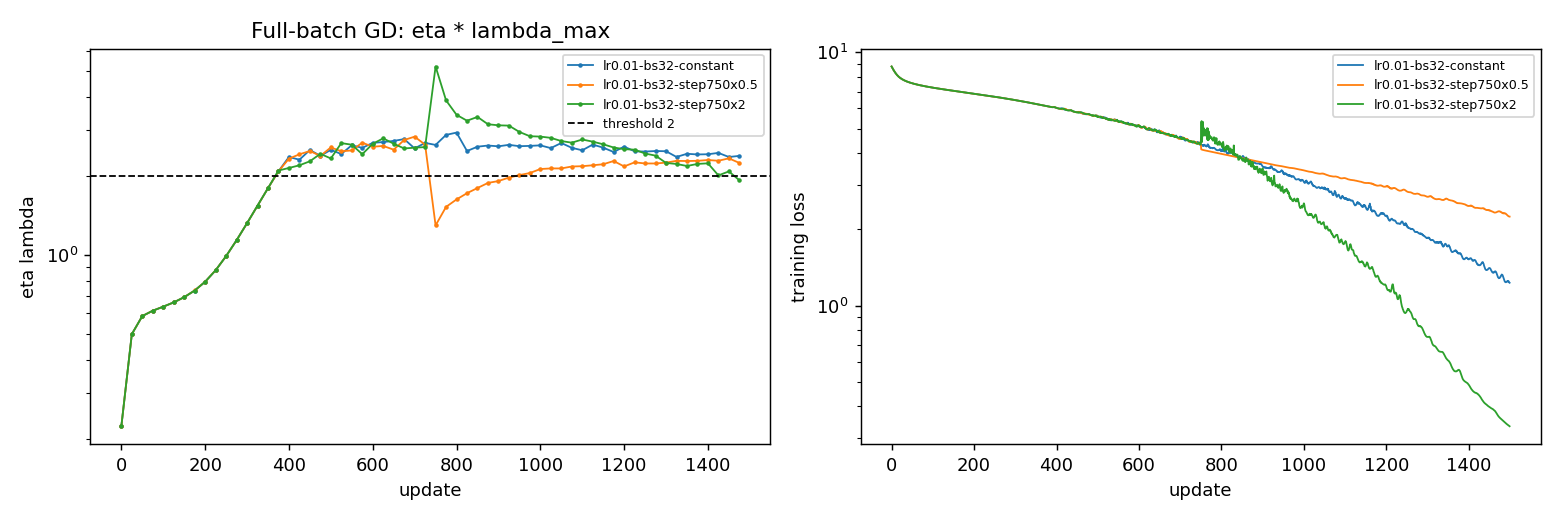
\includegraphics[width=\textwidth]{p3_fullbatch_core.png}
\caption{Left: $\eta\lmax$ (log axis) for the three full-batch runs; dashed line at 2. Right: training loss. The learning rate is halved (orange) or doubled (green) at update 750.}
\end{figure}

\begin{table}[H]\centering\small
\caption{Full-batch runs. ``Crossing'' is the first measured update with $\eta\lmax>2$. ``Plateau'' is the median $\eta\lmax$ from 100 updates after the crossing on. ``Loss up'' is the fraction of updates on which training loss rose, before and after the crossing.}
\begin{tabular}{lcccccc}\toprule
Run & $\eta\lmax$ at 0 & Crossing & Plateau & Loss up before & Loss up after & Final loss\\\midrule
$\eta=0.01$ constant & 0.22 & 375 & 2.56 & 0.00 & 0.39 & 1.23\\
halve $\eta$ at 750 & 0.22 & 375 & 2.24 & 0.00 & 0.24 & 2.25\\
double $\eta$ at 750 & 0.22 & 375 & 2.70 & 0.00 & 0.41 & 0.33\\\bottomrule
\end{tabular}
\end{table}

Yes, sharpness goes to the edge and stays there. $\eta\lmax$ starts at 0.22, rises for 375 updates (progressive sharpening), crosses 2, then hovers between 2.2 and 2.7 for the rest of training instead of continuing up. Before the crossing the loss falls on every single update. After it the loss rises on 24 to 41\% of updates, the small oscillation that keeps $\lmax$ pinned near $2/\eta$.

Halving $\eta$ at 750 halves $\eta\lmax$ to 1.3 at once, because $\lmax$ does not change when $\eta$ does. Then the curvature re-sharpens and is back at 2 by update 950. Doubling $\eta$ sends $\eta\lmax$ to about 6, which is unstable: the loss spikes, and the oscillation drives $\lmax$ down over about 600 updates until $\eta\lmax$ is back near 2.2. Both directions end at the same place. The sharpness tracks $2/\eta$, not the other way round.

The final losses (1.23, 2.25, 0.33) are training loss on 32 memorized sequences and say nothing about generalization. They do show that after the curvature adapts, the doubled learning rate trains much faster.

\subsection*{(b) Minibatch AdamW}
%P3B%

\subsection*{(c) Exploration}
%P3C%

%=====================================================================
\section{Inside the Hessian}

\subsection*{(a) Curvature over training}

We measured the Hessian of the course-supplied AdamW run at 13 checkpoints, from initialization to the end of its 614M-token schedule, on a fixed probe batch. Each measurement is a Lanczos run for the extreme eigenvalues, the top eigenvalue of each parameter family's diagonal block, the family composition of the top eigenvectors, and the Frobenius energy of every block pair.

\begin{table}[H]\centering\small
\caption{Extreme eigenvalues of the full Hessian over training. ``Top family'' is the parameter family that holds most of the top eigenvector's mass.}
\begin{tabular}{rrrrrrrl}\toprule
Step & Tokens & Probe loss & $\|g\|$ & $\lmax$ & $\lmin$ & $|\lmin|/\lmax$ & Top family\\\midrule
0 & 0 & 8.795 & 15.92 & 1431.5 & $-1410.1$ & 0.985 & embedding\\
3 & 0.2M & 8.396 & 11.58 & 1571.7 & $-601.7$ & 0.383 & embedding\\
15 & 1.0M & 6.922 & 0.86 & 53.4 & $-17.5$ & 0.327 & embedding\\
61 & 4.0M & 5.401 & 0.62 & 18.1 & $-1.90$ & 0.105 & embedding\\
153 & 10M & 4.607 & 0.27 & 6.50 & $-0.26$ & 0.039 & head\\
305 & 20M & 4.109 & 0.19 & 4.33 & $-0.07$ & 0.016 & head\\
763 & 50M & 3.574 & 0.12 & 3.02 & $-0.08$ & 0.028 & head\\
1526 & 100M & 3.379 & 0.13 & 2.20 & $-0.06$ & 0.029 & head\\
3052 & 200M & 3.220 & 0.11 & 3.16 & $-0.06$ & 0.020 & head\\
4578 & 300M & 3.135 & 0.11 & 3.74 & $-0.05$ & 0.013 & head\\
6104 & 400M & 3.063 & 0.12 & 4.16 & $-0.04$ & 0.009 & head\\
7630 & 500M & 3.007 & 0.13 & 5.28 & $-0.05$ & 0.009 & head\\
9375 & 614M & 2.947 & 0.13 & 5.97 & $-0.08$ & 0.013 & head\\\bottomrule
\end{tabular}
\end{table}

\begin{figure}[H]\centering
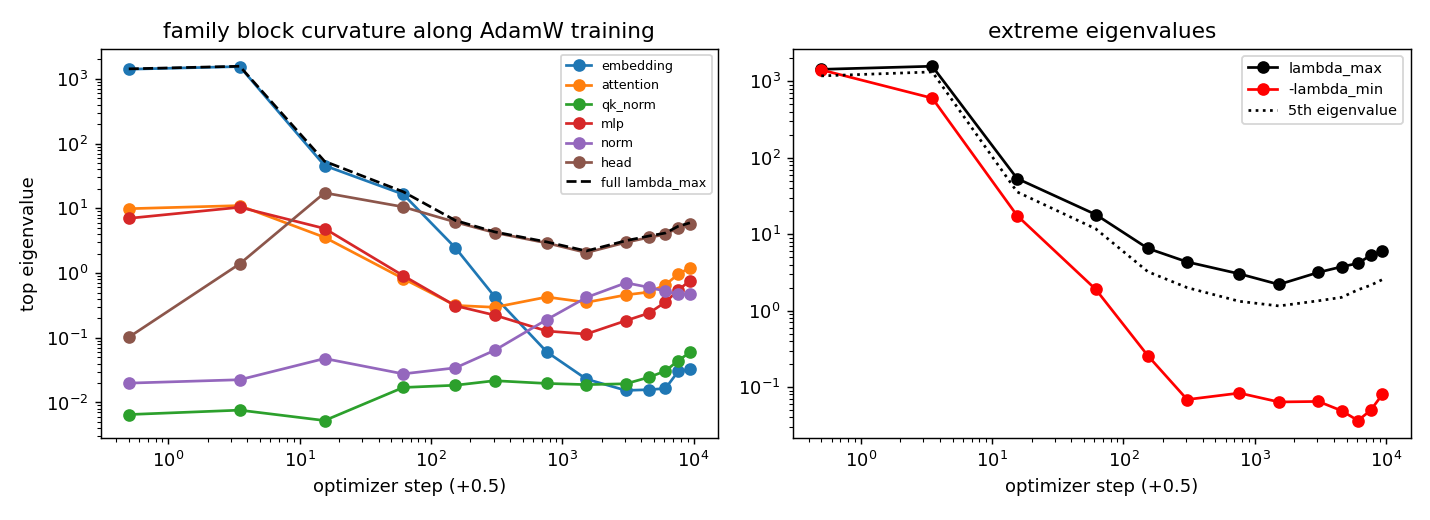
\includegraphics[width=0.49\textwidth]{p4a_curvature.png}
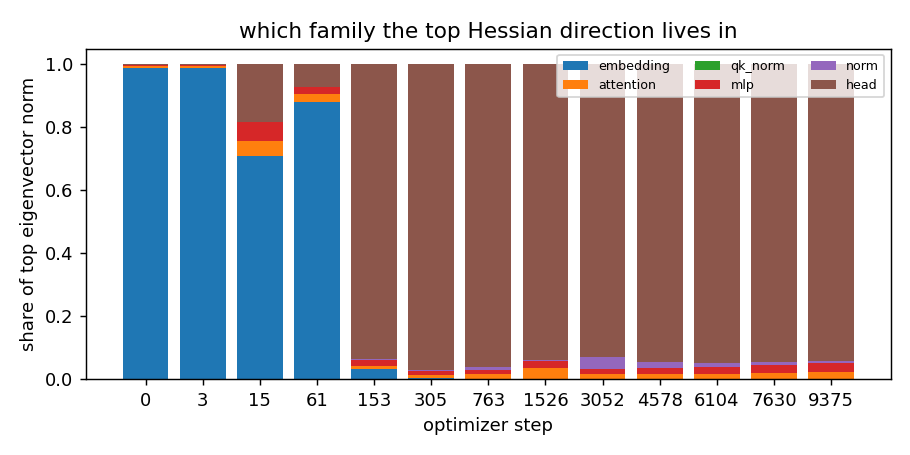
\includegraphics[width=0.49\textwidth]{p4a_top_eigvec.png}
\caption{Left: $\lmax$, $|\lmin|$ and per-family block $\lmax$ over training (log axes). Right: family composition of the top eigenvector.}
\end{figure}

Three phases. At initialization the Hessian is a saddle: $\lmin$ is almost exactly $-\lmax$ and both are about 1400, with 99\% of the top eigenvector in the embedding table. Within 15 steps the embedding block's curvature collapses from 1414 to below 1, and by step 153 it is $0.02$, a drop of five orders of magnitude. Negative curvature disappears at the same time: $|\lmin|/\lmax$ falls below 0.03 after step 153 and stays there.

From step 153 on, the top eigenvector lives in the output head (93 to 97\% of its mass). $\lmax$ keeps falling to a minimum of 2.2 at step 1526, then rises again to 6.0 by the end, a 2.7-fold increase during the linear-decay phase. That rise is the edge of stability seen from the other side: as the learning rate decays the optimizer can tolerate more curvature, and the curvature grows into the room it is given.

The gradient is nearly orthogonal to the top eigenvector after step 153 (overlap below 0.03). Progress happens in directions of low curvature; the sharp direction is where the iterate oscillates, not where it moves.

%P4A_TRACE%

\subsection*{(b) Moving $\lmax$ without moving the loss}
%P4B%

\subsection*{(c) Projected updates}
%P4C%

\end{document}
